% Contribua em https://github.com/gabrielpra1/relatorio-estagio-das
\documentclass[
	% -- opções da classe memoir --
	12pt,				% tamanho da fonte
	openright,			% capítulos começam em pág ímpar (insere página vazia caso preciso)
	oneside,			% Para impressão simples. Para impressão frente e verso, use twoside
	a4paper,			% tamanho do papel.
	% -- opções do pacote babel --
	english,			% idioma adicional para hifenização
	brazil				% o último idioma é o principal do documento
	]{abntex2}
\usepackage{lmodern}			% Usa a fonte Latin Modern
\usepackage[T1]{fontenc}		% Selecao de codigos de fonte.
\usepackage[utf8]{inputenc}		% Codificacao do documento (conversão automática dos acentos)
\usepackage{lastpage}			% Usado pela Ficha catalográfica
\usepackage{indentfirst}		% Indenta o primeiro parágrafo de cada seção.
\usepackage{color}				% Controle das cores
\usepackage{graphicx}			% Inclusão de gráficos
\usepackage{microtype} 			% para melhorias de justificação
\usepackage{listings}
\usepackage{tikz}
\usepackage{float}
\usepackage[brazilian,hyperpageref]{backref}
% Escolha um dos formatos de citação:
% Citação estilo IEEE: "Lorem ipsum [1]."
\usepackage[alf]{abntex2cite}
% \citebrackets[]
% Citação estilo "Lorem ipsum (Autor, 1986)."
% \usepackage[alf]{abntex2cite}	% Citações padrão ABNT
\usepackage{listings}
\definecolor{codegreen}{rgb}{0,0.6,0}
\definecolor{codegray}{rgb}{0.5,0.5,0.5}
\definecolor{codepurple}{rgb}{0.58,0,0.82}
\definecolor{backcolour}{rgb}{0.95,0.95,0.92}
\lstdefinestyle{mystyle}{
  extendedchars=false
  escapeinside="
  backgroundcolor=\color{backcolour},   commentstyle=\color{codegreen},
  keywordstyle=\color{magenta},
  numberstyle=\tiny\color{codegray},
  stringstyle=\color{codepurple},
  basicstyle=\ttfamily\footnotesize,
  breakatwhitespace=false,
  breaklines=true,
  captionpos=b,
  keepspaces=true,
  numbers=left,
  numbersep=5pt,
  showspaces=false,
  showstringspaces=false,
  showtabs=false,
  tabsize=2,
  numberbychapter=false
}
\lstset{style=mystyle}
\renewcommand{\lstlistingname}{Código}
\graphicspath{ {./pictures/} }
\renewcommand{\backrefpagesname}{Citado na(s) página(s):~}
\renewcommand{\backref}{}
\renewcommand*{\backrefalt}[4]{
	\ifcase #1 Nenhuma citação no texto.
	\or Citado na página #2.
	\else Citado #1 vezes nas páginas #2.
	\fi}
\titulo{UMA APLICAÇÃO DE INTELIGÊNCIA COMPUTACIONAL EM PHYTON PARA APOIO AO DIAGNÓSTICO DE CÂNCER DE MAMA}
\autor{Gabriel Del Cesare Barros}
\local{Recife}
\data{2020}
\orientador{Wellington Pinheiro}
\coorientador{} % Deixar vazio caso não haja
\instituicao{
  UNIVERSIDADE FEDERAL DE PERNAMBUCO
  \par
  CENTRO DE TECNOLOGIA E GEOCIÊNCIAS
  \par
  DEPARTAMENTO DE ENGENHARIA BIOMÉDICA}
\tipotrabalho{Trabalho de Conclusão de Curso de Graduação}
\preambulo{}
\definecolor{blue}{RGB}{41,5,195}
\makeatletter
\hypersetup{
    pagebackref=true,
		pdftitle={\@title},
		pdfauthor={\@author},
    	pdfsubject={\imprimirpreambulo},
	    pdfcreator={LaTeX with abnTeX2},
		pdfkeywords={abnt}{latex}{abntex}{abntex2}{trabalho acadêmico},
		colorlinks=true,       % false: boxed links; true: colored links
    	linkcolor=black,     % color of internal links
    	citecolor=blue,      % color of links to bibliography
    	filecolor=magenta,   % color of file links
		urlcolor=blue,
		bookmarksdepth=4
}
% \def\UrlLeft{} \def\UrlRight{} %Contorno dos <links>
\makeatother
\setlength{\parindent}{1.3cm}
\setlength{\parskip}{0.2cm}  % tente também \onelineskip
\makeindex
\begin{document}
\frenchspacing
\renewcommand{\imprimircapa}{
  \begin{capa}
    \center
    \ABNTEXchapterfont\Large\textbf\imprimirinstituicao
    \vspace*{1cm}
    {\ABNTEXchapterfont\large\textbf\imprimirautor}
    \vfill
    \begin{center}
    \ABNTEXchapterfont\bfseries\ \imprimirtipotrabalho \\
    \ABNTEXchapterfont\bfseries\LARGE\imprimirtitulo
    \end{center}
    \vfill
    \large\imprimirlocal, \par
    \large\imprimirdata
    \vspace*{1cm}
  \end{capa}
}
\imprimircapa

\makeatletter
\renewcommand{\folhaderostocontent}{
  \begin{center}
    {\ABNTEXchapterfont\large\textbf\imprimirautor}
    \vspace*{\fill}\vspace*{\fill}
    \begin{center}
    	\ABNTEXchapterfont\bfseries\Large\imprimirtitulo
    \end{center}
    \vspace*{\fill}
    \abntex@ifnotempty{\imprimirpreambulo}{
      \hspace{.45\textwidth}
      \begin{minipage}{.5\textwidth}
      \SingleSpacing
      \imprimirpreambulo
      \par
      {\imprimirorientadorRotulo~\imprimirorientador\par}
      \abntex@ifnotempty{\imprimircoorientador}{
    	{\imprimircoorientadorRotulo~\imprimircoorientador}
      }
      \end{minipage}
      \vspace*{\fill}
    }
    \vspace*{\fill}
    {\large\imprimirlocal}
    \par
    {\large\imprimirdata}
    \vspace*{1cm}
  \end{center}
}


\makeatother
\makeatletter
% \addtocounter{page}{+1}
\begin{center}

Nome do Aluno

\vspace{1cm}

\textbf{Título do Trabalho}

\end{center}

\vspace{.4cm}

\begin{flushright}
\parbox{8cm}{
\singlespacing{Dissertação apresentada, como requisito\linebreak parcial para obtenção do título de Mestre em Ciências, ao Programa de Pós-Graduação em Engenharia Mecânica, da Universidade do Estado do Rio de Janeiro. Área de\linebreak concentração: Fenômenos de Transporte}.
}
\end{flushright}

\vspace{.6cm}


% insira abaixo a data de sua defesa
% Caso não tenha defendido ainda, deixe em branco

\noindent Aprovado em: 29 de Maio de 2012

\noindent Banca Examinadora:


%
%
% Os professores da UERJ DEVEM ser citados primeiro, independente de quem seja o orientador.
%
%



\vspace{.7cm}

\begin{flushright}
\parbox{12cm}{

\singlespacing

\hrulefill \\

\vspace{-.4cm}
Prof. Dr. Nome do Professor 1 (Orientador)
\newline
Instituto de Matemática e Estatística da UERJ
\vspace{.7cm}

\hrulefill \\

\vspace{-.4cm}
Prof. Dr. Nome do Professor 2
\newline
Faculdade de Engenharia da UERJ
\vspace{.7cm}

\hrulefill \\

\vspace{-.4cm}
Prof. Dr. Nome do Professor 3
\newline
Universidade Federal do Rio de Janeiro - UFRJ - COPPE
\vspace{.7cm}

\hrulefill \\

\vspace{-.4cm}
Prof. Dr. Nome do Professor 4
\newline
Instituto de Geociências da UFF
\vspace{.7cm}

\hrulefill \\

\vspace{-.4cm}
Prof. Dr. Nome do Professor 5
\newline
Universidade Federal do Rio de Janeiro - UFRJ - COPPE
\vspace{.7cm}

}
\end{flushright}
\vfill

\begin{center}
Rio de Janeiro\linebreak 2012
\end{center}
% \includepdf{folhadeaprovacao_final.pdf}
\makeatletter
% \begin{dedicatoria}
   \vspace*{\fill}
   \centering
   \noindent
   \textit{Dedicatória: OPCIONAL} \vspace*{\fill}
\end{dedicatoria}


\begin{agradecimentos}
\begin{flushright}
\parbox{0.65\linewidth}{
\itshape \flushright

AGRADECIMENTOS \\
\vspace{0.5 in}
AGRADECIMENTOS \\
\vspace{0.5cm}
AGRADECIMENTOS \\
\vspace{0.5cm}
AGRADECIMENTOS
}
\end{flushright}
\end{agradecimentos}

% \begin{epigrafe}
    \vspace*{\fill}
	\begin{flushright}
		\textit{``Epígrafe (Opcional – NBR10520). 
		Elemento opcional, no qual o autor apresenta uma citação, 
		seguida de indicação de autoria, 
		relacionada à matéria tratada no corpo do trabalho.''}
	\end{flushright}
\end{epigrafe}


\setlength{\absparsep}{18pt} % ajusta o espaçamento dos parágrafos do resumo
\begin{resumo}
	Tendo em vista que a necessidade de um diagnóstico precoce de câncer é primordial para um tratamento efetivo,
e consequentemente a cura da neoplasia,
pesquisa-se sobre o desenvolvimento de uma Inteligência Computacional escrita na linguagem Phyton,
com o intuito de criar um mecanismo de apoio ao diagnóstico médico.
Para tanto, é necessário o desenvolvimento de um script com funções de aprendizado de máquina,
aplicação do banco de dados “Diagnostic Dataset” da Breast Cancer Wisconsi (1992).
Além da utilização de algoritmos computacionais,
que possibilitarão a análise por meio da ferramenta, para que assim,
ela informe se determinado conjunto de atributos tumorais tem alta probabilidade de ser maligno.
Diante disso, após sua execução, verifica-se que o script apresenta, uma acurácia de 96\%,
o que impõe a constatação de que é possível o desenvolvimento de um script que auxilie o diagnóstico médico com uma taxa de exatidão relevante.
\vspace{\onelineskip}

\noindent

\textbf{Palavras-chave:} Inteligência computacional. Apoio ao diagnóstico. Script. Phyton. Câncer de mama.

\end{resumo}
\begin{resumo}[Abstract]
 \begin{otherlanguage*}{english}
	In view of the necessity for early diagnosis of cancer is primordial for effective treatment and,
consequently,
the cure of cancer,
research on the development of a Computational Intelligence written in Phyton language,
in order to create a support mechanism to medical diagnosis.
For this,
it’s necessary to develop a script with machine learning functions,
application of Breast Cancer Wisconsi's “Diagnostic Dataset” (1992).
In addition to the use of computational algorithms,
which will enable analysis through the tool,
so that it can inform if a certain set of tumor attributes is likely to be malignant.
Given this, after its execution, it appears that the script has an accuracy of 96\%,
what imposes the realization that it is possible to develop a script that helps the medical diagnosis with a rate of relevant accuracy.
\vspace{\onelineskip}

\noindent
\textbf{Key-words}: Computational Intelligence. Diagnostic Support. Script. Phyton. Breast Cancer.

 \end{otherlanguage*}
\end{resumo}


% ---
% inserir lista de ilustrações
% ---
\pdfbookmark[0]{\listfigurename}{lof}
\listoffigures*
% OPCIONAL
\cleardoublepage
% ---

\renewcommand{\lstlistlistingname}{Lista de Códigos}
\pdfbookmark[0]{\lstlistlistingname}{lol}
\begin{KeepFromToc}
\lstlistoflistings*
\end{KeepFromToc}
\cleardoublepage

% ---
% inserir lista de tabelas
% ---
\pdfbookmark[0]{\listtablename}{lot}
\listoftables*
% OPCIONAL
\cleardoublepage
% ---

% ---
% inserir lista de abreviaturas e siglas
% ---
\begin{siglas}
  % \item[$t_E$] Tempo expiratório
  % \item[$t_I$] Tempo inspiratório
  \item[UFPE] Universidade Federal de Pernambuco

\end{siglas}
% ---

% ---
% inserir lista de símbolos
% ---
% \begin{simbolos}
%   \item[$ \Gamma $] OPCIONAL
% \end{simbolos}
% ---

\pdfbookmark[0]{\contentsname}{toc}
\tableofcontents*
\cleardoublepage
\textual
\chapter{Introdução}
\label{chapter:introducao}

As neoplasias malignas, também conhecidas como “Câncer” é um conjunto de patologias que, 
de acordo com a ORGANIZAÇÃO MUNDIAL DE SAÚDE (OMS, 2018), 
é a segunda maior causa de óbitos no mundo, 
responsável por 9,6 milhões de mortes, apenas no ano de 2018 %\cite{ESTATISTICACANCER}
.

Tal problema a nível global atrai a atenção para a importância de um diagnóstico precoce, 
o que aumenta a probabilidade de um tratamento eficaz, pois sabe-se que os pacientes que são diagnosticados em estádios tardios, 
podem não responder aos tratamentos curativos.

Para isso, a tecnologia vem sendo utilizada a fim de aprimorar e auxiliar as equipes multidisciplinares de saúde, 
principalmente nos diagnósticos médicos.

E é nesta realidade em que uma ferramenta tecnológica vem sendo cada vez mais estudada e aplicada: 
A Inteligência Computacional.

Esse ramo da ciência da computação aplicado na área de saúde consegue analisar e definir as variáveis de diversas doenças. 
De acordo com Lobo (2017), “A Inteligência Artificial processa esses dados por meio de algoritmos, 
que tendem a se aperfeiçoar pelo seu próprio funcionamento, 
definindo pelo termo em inglês Self-learning e a propor hipóteses diagnósticas cada vez mais precisas.”
%\cite{IAEMSAUDE}

Assim, tendo conhecimento de tais inventos, viu-se a oportunidade da realização de um mecanismo, 
que será apresentado neste trabalho, onde se facilitasse a detecção do câncer, auxiliando os profissionais médicos: 
Uma Inteligência computacional, idealizada em forma de Script, escrita na linguagem Python que, 
a partir de um banco de dados, aprenda como diferenciar se um tumor é maligno ou benigno.

Como base, para “ensinar” a inteligência artificial os atributos de um tumor maligno e de tumores benignos, 
será utilizada a base de dados da “Breast Cancer Wisconsin” intitulada como “Diagnostic Dataset” As informações contidas nessa base, 
servirão de referência para, quando for suposto um caso de tumor ao Script, ele consiga calcular a probabilidade, 
do mesmo ser de caráter maligno.

Essa análise será feita utilizando-se de seis algoritmos de aprendizagem de máquina, que são: “K-Nearest Neighbors; 
Decision Tree; Random Forest; Support Vector Manchine; Naive Bayes e Artificial Neural Network”, eles auxiliarão a inteligência artificial na tomada de decisão do caso proposto.



















\chapter{O Câncer no Mundo}
\label{chapter:o_cancer_no_mundo}

Denominado, também, como neoplasia ou tumor maligno, o câncer é um conjunto de
mais de 100 doenças, em que há um crescimento exacerbado de células em um
determinado tecido. Essas células, por sua vez, podem se espalhar a tal ponto,
que chegam a atingir outros órgãos e tecidos, fenômeno denominado de
“metástase”, demonstrando o poder agressivo dessa classe de patologias \cite{OQUEECANCER}.

Segundo dados divulgados pela IACR, 
era estimado para o ano de $2018$ uma incidência de $18,1$ milhões de novos casos de câncer no mundo.
Também foi datado, no mesmo ano, $9,6$ milhões de óbitos \cite{MOC}, como mostrado na figura \ref{fig:cancerdata}.

\begin{figure}[H]
\begin{center}
\caption{Incidência mundial de câncer}
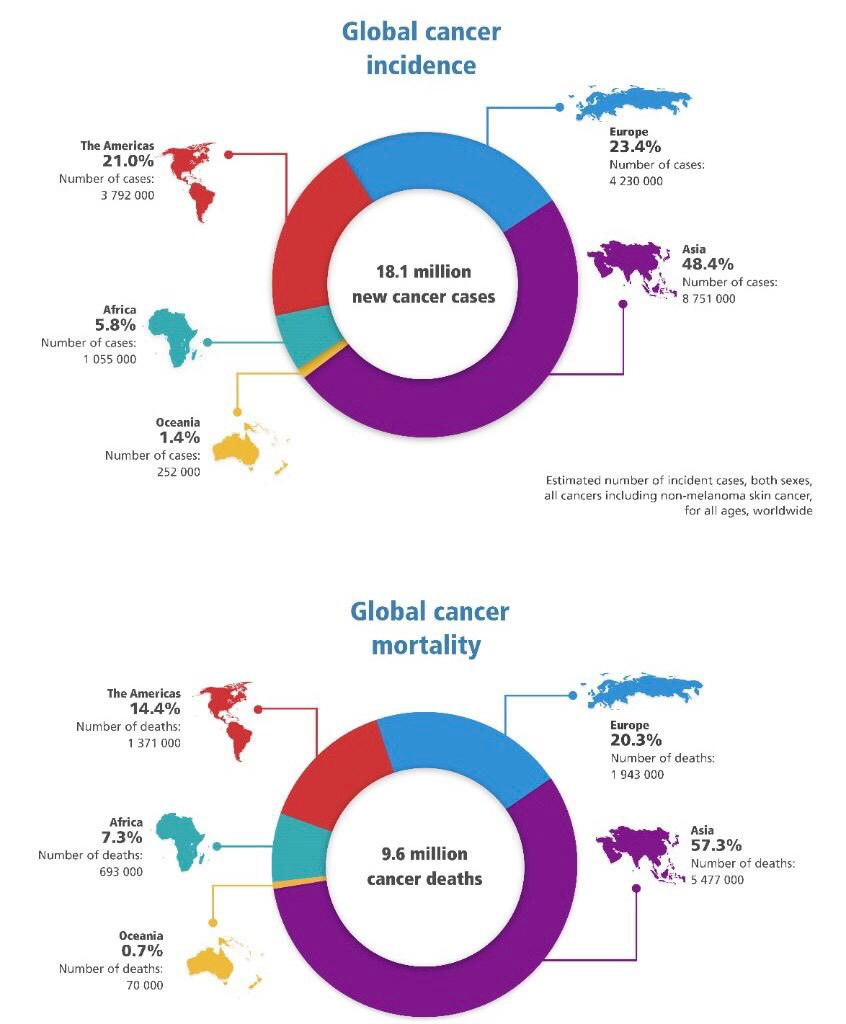
\includegraphics[width=12cm]{cancerdata}
\label{fig:cancerdata}
\end{center}
\legend{Fonte: \url{https://www.iarc.fr/wp-content/uploads/2018/09/Globocan\_01.jpg} \cite{GLOBOCAN} }
\end{figure}

\section{\textbf{Etapas do diagnóstico de câncer}}

O diagnóstico tem como definição ser o processo de identificação a partir de
exames médicos, sintomas e sinais além das amostras do tecido atingido \cite{ATLAS}.

Assim, até que o Patologista, especialista médico responsável pelo laudo anatomopatológico,
faça sua resolução, há alguns processos que auxiliam na análise do problema.
Dentre os exames mais solicitados, está a retirada de um fragmento do tecido suspeito,
para que possa ser feita uma análise em laboratório no microscópio afim de verificar aspecto dos núcleos e
a morfologia das células presentes naquela amostra;
exames de sangue, da medula óssea; radiografia; ultrassonografia, ressonância magnética;
tomografia computadorizada por emissão de pósitrons (PET-TC), são exemplos de exames convencionais \cite{VENCER}.

É importante destacar que a solicitação desses procedimentos irá variar de acordo com a suspeita do tumor,
além da necessidade de uma avaliação mais abrangente,
pois há situações em que os exames convencionais não expõem a informação necessária para um diagnóstico definitivo.
E em alguns casos é preciso a realização de exames Imunohistoquímicos (IHQ), com marcações especiais.

Todo esse processo é de extrema importância, pois, apenas a partir da análise desses laudos,
pelo médico responsável, que ele poderá, confirmar ou descartar a hipótese da neoplasia, e em caso de confirmação,
iniciar um plano de tratamento específico para o problema.


\section{\textbf{Importância do diagnóstico precoce}}

O processo de identificação, exame e avaliação do câncer requer vários fatores, e, portanto, requer tempo.

Porém, profissionais e órgãos da área de saúde alertam para a importância de um diagnóstico precoce,
pois esse, pode elevar as chances de um prognóstico favorável ao paciente.

O Ministério da Saúde do Brasil relata a importância de um diagnóstico em estágios iniciais da seguinte maneira:

“O objetivo do diagnóstico precoce é identificar pessoas com sinais e sintomas iniciais da doença,
primando pela qualidade e pela garantia da assistência em todas as etapas da linha de cuidado da doença.
O diagnóstico precoce, portanto, é uma estratégia que possibilita terapias mais simples e efetivas,
ao contribuir para a redução do estágio de apresentação do câncer.
Assim, é importante que a população em geral e os profissionais de saúde reconheçam os sinais de alerta dos cânceres mais comuns,
passíveis de melhor prognóstico se descobertos no início.
A maioria dos cânceres é passível de diagnóstico precoce mediante avaliação e encaminhamento após os primeiros sinais e sintomas.”
\cite{DIAGNOSTICO}.


\chapter{Inteligência Computacional e Saúde}
\label{chapter:inteligencia_computacional_e_saude}

A inteligência Computacional é uma ferramenta de computação que automatiza processos complexos,
como por exemplo a identificação e categorização de imagens. E já tem muito espaço na saúde,
uma área de extrema relevância à sociedade, que requer atenção e agilidade, pois cuida das diversas aplicações neste ramo, estão:

\begin{itemize}
\item Tratamento de doenças: Se refere a capacidade dos computadores de auxiliar no tratamento das patologias.
  Por exemplo o “Watson”, algoritmo desenvolvido pela IBM,
    que informa os vários tratamentos possíveis para cada caso, informando efeitos colaterais e o grau de risco de cada uma.

\item Acurácia no resultado de exames: Existem algoritmos computacionais,
  atualmente, que conseguem ser mais precisos em comparação à alguns exames médicos,
    por exemplo um algoritmo desenvolvido na Alemanha, EUA e China,
    que superou especialistas em retina na identificação de diagnósticos no exame de tomografia óptica

\item Correlação de sintomas: O TensorFlow, por exemplo,
  uma biblioteca desenvolvida pela Google, consegue identificar retinopatia diabética através de semelhança de imagens,
    e consegue fazer associação de sintomas com taxa de acerto semelhante aos especialistas da área.

\item Recuperação de dados: A partir da memória da IC,
  facilita-se a recuperação dos arquivos com os dados e ficha médica dos pacientes, quando houver necessidade.

\item Alertas de emergência: Pode-se criar alertas sobre mudanças no quadro dos pacientes,
  os enviando ao profissional responsável, sendo de extrema importância principalmente em emergências.
\end{itemize}

Para o desenvolvimento da Inteligência Computacional, por meio do Script, que auxiliará na avaliação médica,
foram utilizadas as seguintes ferramentas:

\section{\textbf{Phyton}}

Python é uma linguagem de programação, no ranking das mais utilizadas do mundo, ela foi criada por Guido Van Rossum,
com o objetivo de proporcionar produtividade e legibilidade na realização de projetos computacionais \cite{PYTHON}.

A sua sintaxe é simples, sendo comparada até a um pseudocódigo executável.
Usa a chamada “Identação”, que é um recuo no código, em relação a sua margem, para marcar blocos.
Também é uma linguagem de baixo uso de caracteres especiais e palavras chaves.

Apesar de ser uma linguagem comumente utilizada para IC,
ainda não é simples de encontrar artigos e documentos que instruam para a realização de um programa básico,
a fim de iniciar os primeiros passos na área

Assim, será utilizado no Script de Câncer de mama as seguintes ferramentas básicas e de fácil acesso:

\begin{itemize}
\item Pandas - é uma biblioteca do Python,
  que fornece ferramentas de análise e estruturas de dados de alta performance e de simples utilização \cite{PANDAS}.
\item Scikit-learn - é outra biblioteca do Python que inclui alguns algoritmos de classificação, regressão e agrupamento \cite{SCIKIT}.
\end{itemize}

\section{\textbf{A base de dados}}

Para comprovar a correlação do diagnóstico de câncer a partir dos parâmetros dos exames,
e ensinar a inteligência computacional a tentar descobrir o provável diagnóstico,
foi-se utilizado uma base de dados de autoria da “Breast Cancer Wisconsin” chamada por eles como “Diagnostic Dataset”, presente no site:
(\url{https://www.kaggle.com/uciml/breast-cancer-wisconsin-data})\cite{BREASTCANCER}.

É um conjunto de registros de resultados de exames utilizados para detecção do Câncer de mama,
comumente utilizada para aprendizado e aplicações reais.
Ela foi criada em 1995 por Dr. William H. Wolberg, W. Nick Street e Olvi L. Mangasarian na universidade de Wisconsin.

Possui 569 instâncias, que estão correlacionadas com as pessoas que participaram da coleta.
E 32 tipos de atributos que são os dados coletados de cada análise.
Entre os atributos está o diagnóstico final dado pelo médico informando se o tumor é maligno ou benigno.

Os dados dessa base foram obtidos através de diversos procedimentos de diagnóstico médico.
Dentre eles, há a imagem digitalizada de um aspirado por agulha fina (PAAF)
de um tecido mamário que tem como função determinar os aspectos dos núcleos celulares presentes no tecido.

Essa base é importante para o desenvolvimento do Script do Câncer de mama
pois ela permite analisar os atributos coletados para ensinar a inteligência computacional a tentar descobrir o provável diagnóstico.

Os atributos coletados na base de dados determinam as características do tumor maligno, como:

Raio, textura, perímetro, área, suavidade, compacidade, concavidade e os pontos côncavos presentes;
simetria, além da dimensão fractal.
Para cada um desses parâmetros foram analisados a média, erro padrão e o ``pior'' ou mais largo (média dos 3 maiores valores).



\chapter{Os Métodos de Análise}
\label{chapter:os_metodos_de_analise}

\section{\textbf{K-nearest Neighbors}}

Existem vários métodos de análise de algoritmos, um dos mais simples é o “K-Nearest Neighbors”, utilizado no Script, que funciona da seguinte forma:

Observando a imagem abaixo, observa-se um gráfico com um conjunto de bolas amarelas e roxas; também é possível perceber uma bola desconhecida, destacada na cor vermelha. Para calcular se ela é roxa ou amarela, o algoritmo do KNN determinará a sua cor, de acordo com as N bolas mais próximas.

Por exemplo, caso N seja igual a 3, a bola desconhecida será classificada como roxa e no caso de N igual à 6 será classificada como amarela:

\begin{figure}[!htb]
\begin{center}
\caption{K-nearest Neighbors}
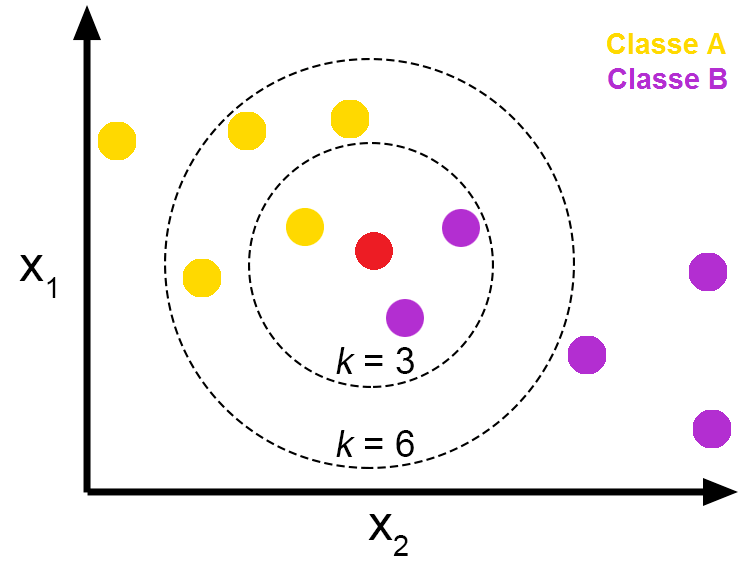
\includegraphics[width=8cm]{knearestneighbors}
\end{center}
\legend{Fonte: https://miro.medium.com/max/1506/0*jqxx3-dJqFjXD6FA}
\cite{KNN}
\end{figure}




\section{\textbf{Decision tree}}

A chamada “Árvore de Decisão”, define um novo elemento com base em rotinas pré-estabelecidas. Por exemplo, se há um banco de dados de pessoas que foram jogar tênis com base na situação do clima, pode-se chegar a seguinte árvore de decisão:


\begin{figure}[!htb]
\begin{center}
\caption{Decision Tree}
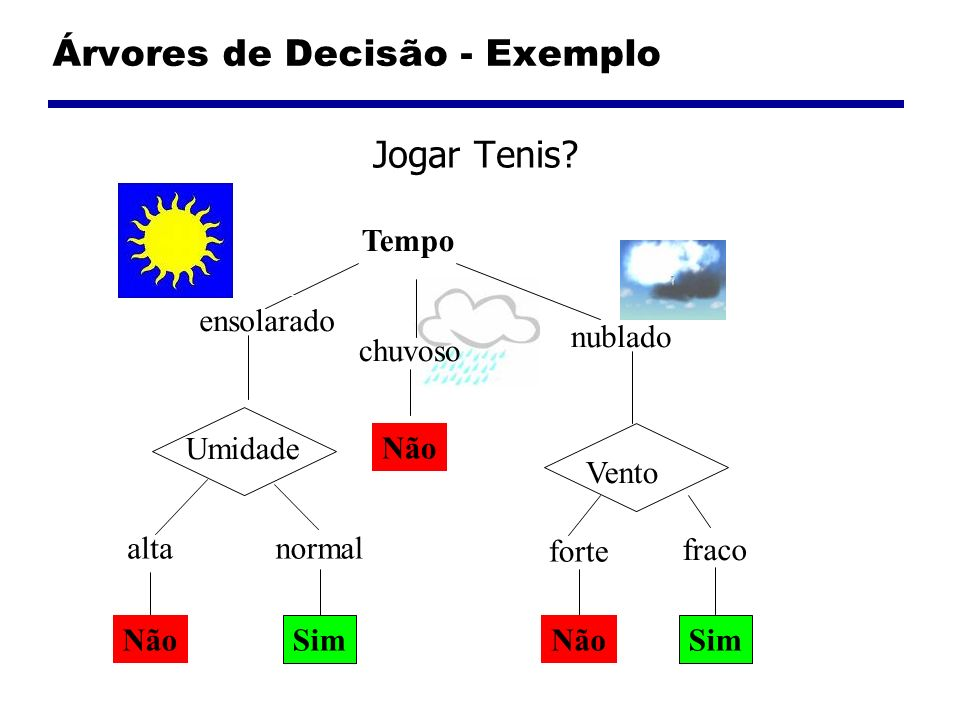
\includegraphics[width=8cm]{decisiontree}
\end{center}
\legend{Fonte: https://slideplayer.com.br/slide/358847/2/images/5/\%C3\%81rvores+de+Decis\%C3\%A3o+-+Exemplo.jpg}
%\cite{ARVOREDECISAO}
\end{figure}

E então quando alguém perguntar se haverá jogo de tênis no dia, ela responderá de acordo com o clima, seguindo a árvore de decisão.

\section{\textbf{Random Forest}}

Algoritmo que cria várias árvores de decisões, definido anteriormente, e as combinam para obter uma predição com maior acurácia e mais estável:



\begin{figure}[!htb]
\begin{center}
\caption{Random Forest}
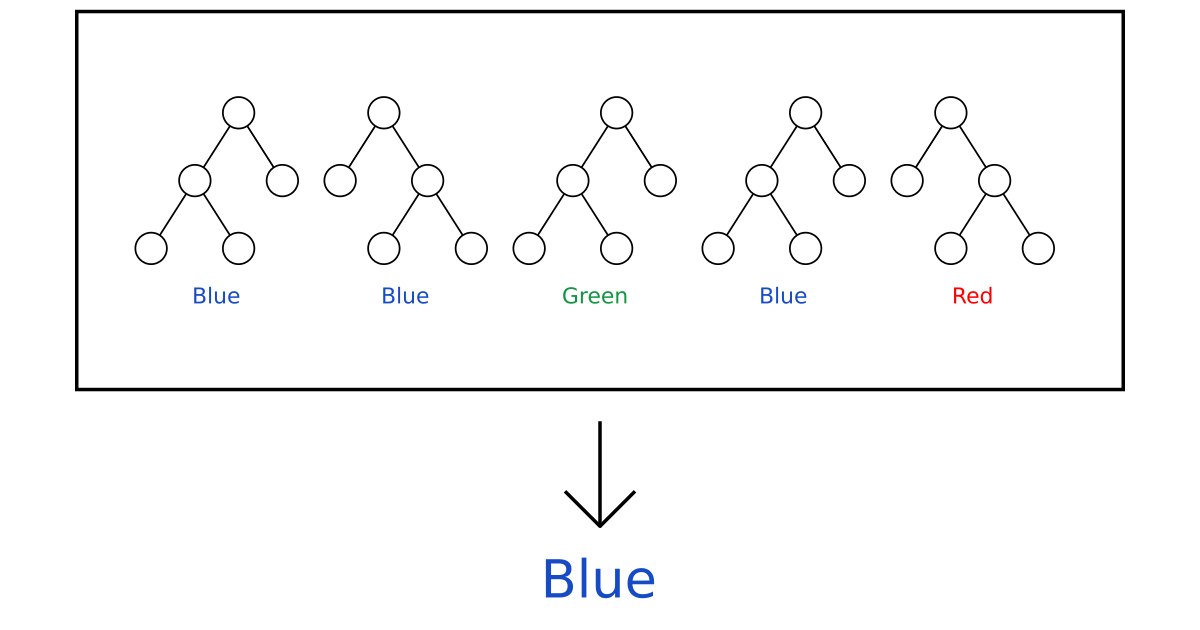
\includegraphics[width=8cm]{randomforest}
\end{center}
\legend{Fonte: https://victorzhou.com/media/random-forest-post/random-forest.png}
\cite{RANDOMFOREST}
\end{figure}



\section{\textbf{Support Vector machine}}

O classificador intitulado de “Máquina de Vetores de Suporte” categoriza, com base em uma divisão dos dados.  

Por exemplo, na imagem abaixo, há quadrados e círculos de cores vermelhas e azuis, respectivamente. 
Pode-se dividi-las com qualquer uma das retas do quadrante esquerdo. 
Porém, como mostrado no quadrante direito, 
há uma única reta em que a sua distância em relação a figura azul mais próxima é igual a distância da figura vermelha mais próxima, 
logo se encontra a melhor reta para separá-las.


\begin{figure}[!htb]
\begin{center}
\caption{Suport Vector Machine}
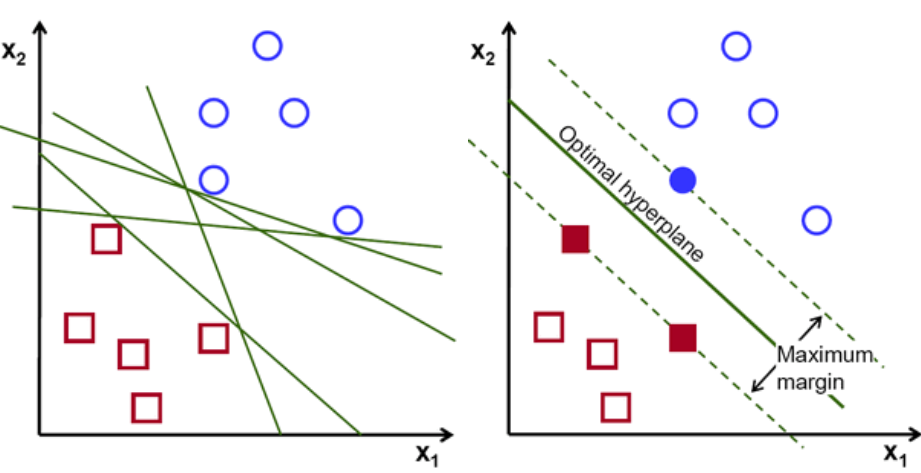
\includegraphics[width=8cm]{suportvectormachine}
\end{center}
\legend{Fonte: https://miro.medium.com/max/921/1*nUpw5agP-Vefm4Uinteq-A.png}
\cite{SVM}
\end{figure}

Em casos mais complexos utilizam-se hiperplanos.


\section{\textbf{Naive bayes}}

O classificador “Naive Bayes” é baseado no Teorema de Bayes. Ele desconsidera a correlação entre as variáveis, e por isso é chamado de “ingênuo”. 

Um exemplo de sua utilização seria para considerar se um fruto qualquer é uma maçã, assim, analisa-se se ele é vermelho, redondo e de aproximadamente 3 polegadas (Características da fruta colocada em exemplo). De acordo com o Teorema de Bayes, cada um desses fatores contribui independentemente para a probabilidade de que este fruto seja realmente uma maçã.

Quando se lida com muitos dados, sendo eles todos independentes, assumisse que distribuição ocorre de acordo com uma gaussiana simples, por isso usa-se o classificador GauissanNB para calculá-lo.


\begin{figure}[!htb]
\begin{center}
\caption{Naive Bayes}
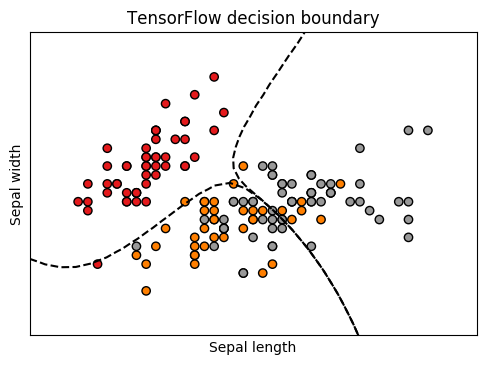
\includegraphics[width=8cm]{naivebayes}
\end{center}
\legend{Fonte: https://nicolovaligi.com/tf\_iris.png}
\cite{NAIVEBAYES}
\end{figure}


\section{\textbf{Artificial Neural Network}}

A chamada, “Rede neural artificial” é um classificador que se baseia no sistema de redes neurais que utiliza o mecanismo de aprendizagem de pesos sinápticos de tal forma que a unidade de saída produza as respostas corretas para cada exemplo, realizando atualizações de forma dinâmica e interativa até chegar aos pesos corretos.

É a mais parecida, com o sistema que ocorre no cérebro:


\begin{figure}[!htb]
\begin{center}
\caption{Artificial Neural Network}
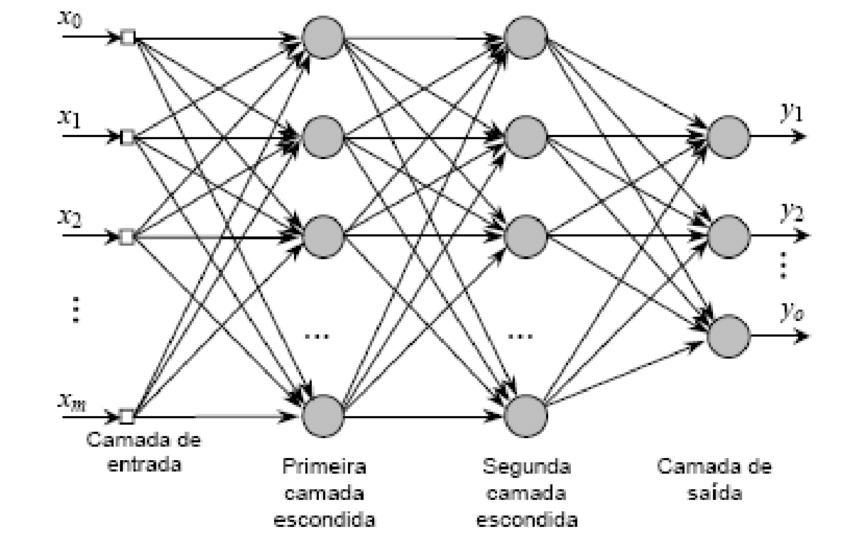
\includegraphics[width=8cm]{mlp}
\end{center}
\legend{Fonte: https://www.researchgate.net/profile/Anderson\_Oliveira6/publication/240772105/figure/fig2/AS:667857415319554@1536241024122/Figura-1-Rede-Neural-Artificial-Multicamadas.png}
\cite{MLP}
\end{figure}



\chapter{O Script do Câncer de Mama}
\label{chapter:o_script_do_cancer_de_mama}


Não foi exposto aqui o código final inteiro, por ser bastante extenso, encontra-se ao final do trabalho no apêndice \ref{app:code}, seção
\ref{lst:code}, página \pageref{lst:code}, para quem se interessar, ler melhor.

As funções que se referem ao aprendizado de máquina são a parte principal do código e onde pode haver dúvidas quanto a sintaxe.
Portanto será explicado na seção \ref{sintaxe}.

Para executar o script, precisa ter o python \cite{PYTHON} instalado,
e então salvar o conteúdo do código no apêndice \ref{app:code} em um arquivo, por exemplo ``script.py'',
e colocar na mesma pasta do arquivo com o banco de dados
(\url{https://www.kaggle.com/uciml/breast-cancer-wisconsin-data/download}) \cite{BREASTCANCER}.
Em seguida, no local onde estão os arquivos executa-se:

\begin{lstlisting}[language=Python, caption=Executar Script.py]
python script.py
\end{lstlisting}

\section{Validação Cruzada}

Antes de ir diretamente ao código, é necessário a compreensão da validação cruzada.
A validação cruzada é um método de aprendizado de máquina em que utiliza-se uma
porcentagem para teste e outra para treinamento, comumente $10\%$ para testes e $90\%$ para treinamento.
Desta forma o script treina de diferentes formas melhorando sua confiabilidade.


Por exemplo, na figura \ref{fig:crossvalidation}, a base de dados foi dividida em 6,
e em cada iteração usa-se uma parte diferente como teste, e o restante para o treinamento.

\begin{figure}[H]
\begin{center}
\caption{Validação Cruzada}
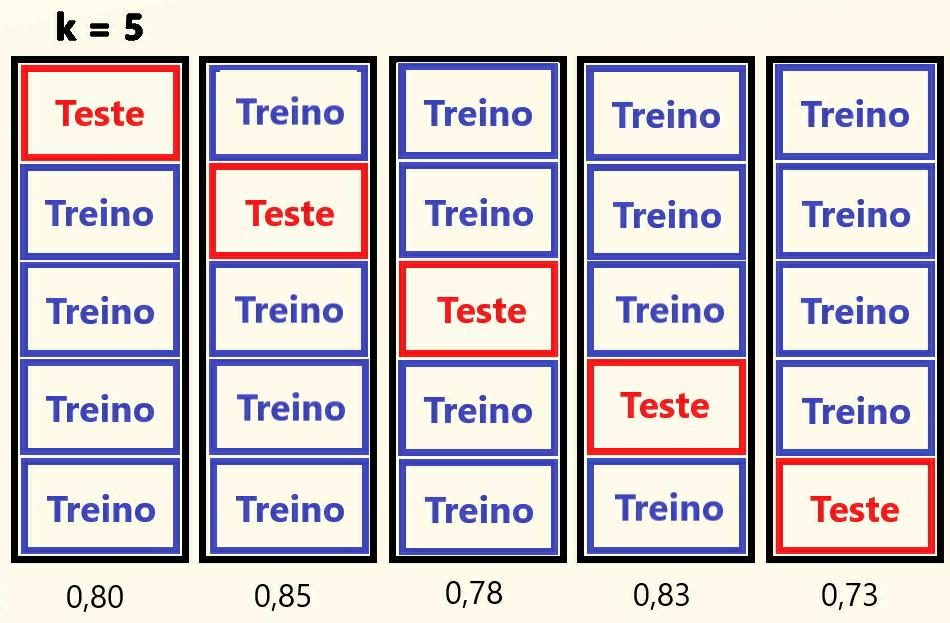
\includegraphics[width=12cm]{crossvalidation}
\label{fig:crossvalidation}
\end{center}
\legend{Fonte: \url{https://didatica.tech/wp-content/uploads/2019/10/Kfold_Resultados.png} \cite{CROSSVALIDATION} }
\end{figure}

\section{Sintaxe}
\label{sintaxe}
Primeiramente será explicada a função ``Máquina de Vetor de Suporte'',
ela é chamada na primeira linha do código \ref{alg:simples}.

Na segunda linha é chamada a validação cruzada $cros\_val\_score$ que salva na variável $scores$ um vetor com a acurácia das $10$ iterações.
Na terceira e quarta linha, informa na tela a média dos valores das acurácias.
A quinta, sexta e sétima servem para ao final do script, informar qual foi a função com o melhor desempenho.

\begin{lstlisting}[language=Python, caption=Sintaxe Simples, label=alg:simples]
svm = SVC(kernel='poly',degree=1)
scores = cross_val_score(svm, X, y, cv=10, scoring='accuracy')
function_print = 'SuppotVectorMachine:\t' + str(scores.mean())
print(function_print)
if scores.mean() > best_score:
  best_score = scores.mean()
  best_function=function_print
\end{lstlisting}

Por último será mostrada a função ``Árvore de decisão'' no código \ref{alg:parametro},
pois ela possui um parâmetro $max\_depth=n$ que pode variar,
e deseja-se saber para qual $n$ ela consegue a melhor acurácia.

Para isso o $n$ será variado de $1$ a $9$, como mostra as linhas $1$ e $2$.
As linhas $5$, $6$ e $7$ salvam o $n$ com a maior acurácia juntamente com o resultado.
O restante é igual ao código \ref{alg:simples}.

\begin{lstlisting}[language=Python, caption=Sintaxe com Parâmetro, label=alg:parametro]
max_score = 0
for n in range(1,10):
  tree = DecisionTreeClassifier(max_depth=n, random_state=0)
  scores = cross_val_score(tree, X, y, cv=10, scoring='accuracy')
  if  scores.mean() > max_score:
    max_score = scores.mean()
    max_n = n
function_print = 'DecisionTreeClassifier:\t' + str(max_score) + '\t(max_depth=' + str(max_n) + ')'
print(function_print)
if max_score > best_score:
  best_score = max_score
  best_function=function_print
\end{lstlisting}

Assim o script consegue definir a melhor função e parâmetro a partir da acurácia, em determinar se o tumor é maligno ou benigno.


E sua execução resultou nos dados encontrados na tabela \ref{tab:resultado}.

\setlength{\arrayrulewidth}{0.6mm}
\begin{table}[h!]
\centering
\begin{tabular}{ |c|c|c| }
 \hline
 Função                   & Acurácia           & Parâmetro  \\
 \hline
 KneighborsClassifier     & 0.9297619047619048 & n\_neighbors = 8  \\
 DecisionTreeClassifier   & 0.9280701754385964 & max\_depth = 5    \\
 RandomForestClassifier   & 0.9649122807017543 & max\_depth = 80   \\
 SuppotVectorMachine      & 0.9051065162907269 &                   \\
 GaussianNB               & 0.9367794486215537 &                   \\
 MLPClassifier            & 0.8963032581453634 &                   \\
 \hline
 \hline
 \multicolumn{3}{|c|}{ Melhor Função} \\
 \hline
 RandomForestClassifier:  & 0.9649122807017543 & max\_depth = 80   \\
 \hline
\end{tabular}
  \caption{Resultado Final}
\label{tab:resultado}
\end{table}

Observa-se pelos resultados na tabela que com esse código simples, consegue-se uma acurácia de $96\%$
utilizando o classificador ``Floresta Aleatória'' com $max\_depth=80$.









\chapter{Conclusão}
\label{chapter:conclusao}

CONCLUSÃO

\pagebreak
\chapter{Trabalhos Futuros}
\label{chapter:trabalhos_futuros}

Para os desenvolvimentos de novos trabalhos na área, sugere-se, o desenvolvimento de um reprodutor gráfico para demonstrar os resultados do Script de forma mais prática, e de fácil acesso, por exemplo uma interface web. 

Em relação ao código desenvolvido nesse trabalho, um outro tipo de abordagem seria sua aplicação para outras doenças, como Hipertensão, Diabetes, que tem como base para seu diagnóstico exames que características padrões.

Em relação às linguagens de programação, a Golang \cite{GO} apresenta uma maior velocidade, ao ser confrontado com outros programas já desenvolvidos, pois possui características estruturais únicas que lhe proporcionam essa vantagem. Também poderia ser utilizado o Javascript \cite{JAVASCRIPT}, levando em consideração que ele é conhecido a nível mundial, de acordo com estatísticas pois possui características únicas como frontend web, o que em sua maioria, atrai mais o público.

Portanto, há muito o que se desenvolver no campo de Inteligência Artificial voltado à Engenharia Biomédica, auxílio ao diagnóstico de outras doenças e análise de exames.

\phantompart
\postextual
\bibliography{bibliography}
\begin{apendicesenv}
  \chapter{O Código}
  \lstinputlisting[language=Python, caption=Código Final, label=lst:code]{../code/script.py}
  \label{app:code}
\end{apendicesenv}

% \begin{anexosenv}
\chapter{Título Opcional.}
Documentos não elaborados pelo autor, utilizados de fundamentação (mapas, leis, estatutos).
\end{anexosenv}

\phantompart
\printindex
\end{document}
